% Options for packages loaded elsewhere
\PassOptionsToPackage{unicode}{hyperref}
\PassOptionsToPackage{hyphens}{url}
%
\documentclass[
]{article}
\usepackage{amsmath,amssymb}
\usepackage{iftex}
\ifPDFTeX
  \usepackage[T1]{fontenc}
  \usepackage[utf8]{inputenc}
  \usepackage{textcomp} % provide euro and other symbols
\else % if luatex or xetex
  \usepackage{unicode-math} % this also loads fontspec
  \defaultfontfeatures{Scale=MatchLowercase}
  \defaultfontfeatures[\rmfamily]{Ligatures=TeX,Scale=1}
\fi
\usepackage{lmodern}
\ifPDFTeX\else
  % xetex/luatex font selection
\fi
% Use upquote if available, for straight quotes in verbatim environments
\IfFileExists{upquote.sty}{\usepackage{upquote}}{}
\IfFileExists{microtype.sty}{% use microtype if available
  \usepackage[]{microtype}
  \UseMicrotypeSet[protrusion]{basicmath} % disable protrusion for tt fonts
}{}
\makeatletter
\@ifundefined{KOMAClassName}{% if non-KOMA class
  \IfFileExists{parskip.sty}{%
    \usepackage{parskip}
  }{% else
    \setlength{\parindent}{0pt}
    \setlength{\parskip}{6pt plus 2pt minus 1pt}}
}{% if KOMA class
  \KOMAoptions{parskip=half}}
\makeatother
\usepackage{xcolor}
\usepackage{graphicx}
\makeatletter
\def\maxwidth{\ifdim\Gin@nat@width>\linewidth\linewidth\else\Gin@nat@width\fi}
\def\maxheight{\ifdim\Gin@nat@height>\textheight\textheight\else\Gin@nat@height\fi}
\makeatother
% Scale images if necessary, so that they will not overflow the page
% margins by default, and it is still possible to overwrite the defaults
% using explicit options in \includegraphics[width, height, ...]{}
\setkeys{Gin}{width=\maxwidth,height=\maxheight,keepaspectratio}
% Set default figure placement to htbp
\makeatletter
\def\fps@figure{htbp}
\makeatother
\setlength{\emergencystretch}{3em} % prevent overfull lines
\providecommand{\tightlist}{%
  \setlength{\itemsep}{0pt}\setlength{\parskip}{0pt}}
\setcounter{secnumdepth}{-\maxdimen} % remove section numbering
\ifLuaTeX
  \usepackage{selnolig}  % disable illegal ligatures
\fi
\IfFileExists{bookmark.sty}{\usepackage{bookmark}}{\usepackage{hyperref}}
\IfFileExists{xurl.sty}{\usepackage{xurl}}{} % add URL line breaks if available
\urlstyle{same}
\hypersetup{
  pdftitle={Trabajo Sistemas de Gestión de la Información Lenguaje de Marcas.},
  pdfauthor={Sidney Silva Braz de Oliveira - 1º DAW},
  hidelinks,
  pdfcreator={Sidney Silva Braz de Oliveira}}

\title{\Huge Trabajo Sistemas de Gestión de la Información Lenguaje de
Marcas.}
\author{Sidney Silva Braz de Oliveira - 1º DAW}
\date{\today}

\begin{document}
\maketitle

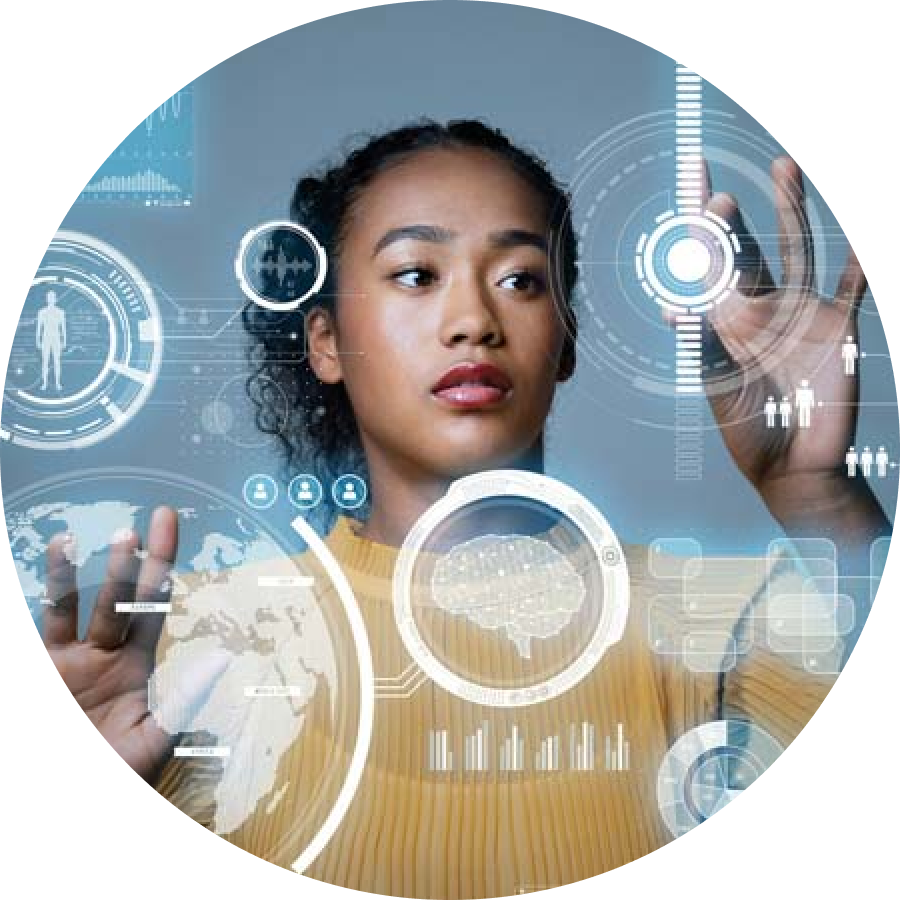
\includegraphics{./SGI.png}


\hypertarget{quuxe9-es-un-sistema-de-gestiuxf3n-de-la-informaciuxf3n}{%
\section{¿Qué es un Sistema de Gestión de la
Información?}\label{quuxe9-es-un-sistema-de-gestiuxf3n-de-la-informaciuxf3n}}

Un \textbf{Sistema de Gestión de la Información}, o Managment
Information System (MIS) en inglés, es una herramienta o software que
permite controlar todos los aspectos de una empresa, ya sean pedidos,
producción, administración, facturación, etc. Gracias a esto, són
\textbf{herramientas perfectas para conseguir unos elevados niveles de
control y calidad}.

Estos sistemas no están pensados solo para grandes empresas. También
permiten a las pequeñas y medianas empresas aprovechar mejor sus
características para conseguir un perfecto conocimiento del
funcionamiento interno, detectando posibles puntos débiles en la gestión
y facilitando la labor de corrección de los mismos.

\hypertarget{cuxf3mo-funcionan}{%
\subsection{¿Cómo funcionan?}\label{cuxf3mo-funcionan}}

Estos recopilan datos para que después seán almacenados, procesados y
finalmente, presentados a los gestores de información de manera
analítica para que hagan su trabajo de ver los puntos a mejorar de la
empresa.

\hypertarget{condiciones-para-el-tratamiento-de-la-informaciuxf3n.}{%
\subsection{Condiciones para el tratamiento de la
información.}\label{condiciones-para-el-tratamiento-de-la-informaciuxf3n.}}

Las condiciones para el correcto tratamiento de la información en el
sistema són:

\begin{itemize}
\tightlist
\item
  La información deberá ser íntegra y adecuada.
\item
  La información estará disponible en el momento oportuno.
\item
  La información deberá ser fiable.
\item
  El tratamiento de la información deberá ser económico.
\item
  La información deberá ser adaptable a las necesidades cambiantes de
  información de los usuarios.
\end{itemize}

\hypertarget{caracteruxedsticas.}{%
\subsection{Características.}\label{caracteruxedsticas.}}

Las características principales de un sistema de gestión de la
información són:

\begin{itemize}
\tightlist
\item
  Produce reportes (anuales, semestrales, trimestrales y mensuales) con
  un formato preestablecido.
\item
  Produce consultas impresas o en pantalla.
\item
  Utiliza datos internos de la empresa, almacenadolos dentro de la base
  de datos de los sistemas de datos transaccionales.
\end{itemize}

\begin{center}\rule{0.5\linewidth}{0.5pt}\end{center}

\hypertarget{planificaciuxf3n-de-recursos-empresariales.}{%
\section{Planificación de recursos
empresariales.}\label{planificaciuxf3n-de-recursos-empresariales.}}

La \textbf{planificación de recursos empresariales o Enterprise Resource
Planning en inglés,} es un sistema que ayuda a automatizar y administrar
los procesos empresariales de una empresa, como pueden ser las finanzas,
la fabricación, recursos humanos, etc.

\hypertarget{caracteruxedsticas-de-un-erp.}{%
\subsection{Características de un
ERP.}\label{caracteruxedsticas-de-un-erp.}}

Las características principales de un sistema de planificación de
recursos empresariales són:

\begin{itemize}
\tightlist
\item
  Acceso a una base de datos centralizada.
\item
  Captura de datos de manera automática.
\item
  Son configurables, por lo que se adaptan a las necesidades de la
  empresa.
\item
  La estructura del trabajo se divide en módulos
\item
  Interacción entre los componentes del ERP.
\item
  Requiere un trabajo de sincronización entre departamentos y
  conocimiento de la herramienta.
\end{itemize}

\hypertarget{tipos-de-erp.}{%
\subsection{Tipos de ERP.}\label{tipos-de-erp.}}

Existen diferentes tipos de ERP si atendemos a dos parámetros;
l\textbf{as necesidades de gestión en empresa} y el \textbf{tipo de
tecnología utilizada por el proveedor ERP.}

\hypertarget{seguxfan-las-necesidades-de-gestiuxf3n.}{%
\subsubsection{Según las necesidades de
gestión.}\label{seguxfan-las-necesidades-de-gestiuxf3n.}}

Existen dos tipos: el \textbf{ERP horizontal} y el \textbf{ERP
vertical}:

\begin{itemize}
\item
  \textbf{ERP Horizontal.} Este tipo de sistema \textbf{cubre los
  procesos de gestión habituales de cualquier empresa.} La mayoria de
  las empresas suelen gestionar cobros, pagos, clientes, proveedores y
  empleados. En este sentido, un \textbf{ERP Horizontal} recogerá
  funcionalidades tales como la contabilidad, el marketing, las
  finanzas, producción, recursos humanos, etc. También puede optimizar
  los procesos de una empresa de manera integral, a lo largo de su
  cadena de valor, o solo en algunas áreas o departamentos concretos.
\item
  \textbf{ERP Vertical.} Este tipo de sistema \textbf{está diseñado para
  un sector en concreto}. Además de contar con todos los módulos básicos
  de un ERP Horizontal, también incluye características añadidas para
  los procesos específicos de cada sector, con lo que su funcionalidad
  mejora. Dependiendo del proveedor, estos sistemas pueden implicar
  gastos mayores y un mayor mantenimiento; pero son desventajas menores
  teniendo en cuenta los beneficios que estos nos pueden aportar.
\end{itemize}

\hypertarget{seguxfan-la-tecnologuxeda-del-proveedor.}{%
\subsubsection{Según la tecnología del
proveedor.}\label{seguxfan-la-tecnologuxeda-del-proveedor.}}

Según la tecnología del proveedor, existen 2 tipos: \textbf{ERP
estándar} y \textbf{EPR personalizable:}

\begin{itemize}
\item
  \textbf{ERP estándar.} Este tipo de sistema contiene funcinalidades
  \textbf{rígidas y preestablecidas.} Son sistemas de rápida
  implementación, desarrollados por grandes fabricantes y garantizan la
  innovación constante del producto pero no son fáciles para adaptarse y
  cualquier personalización, implicará costos y tiempos significativos.
\item
  \textbf{ERP personalizable.} Este tipo de sistema está adaptado a los
  requerimientos de la empresa, diseñado a su propia imagen y semejanza
  y tiene en cuenta las necesidades de esta. También incluye una
  \textbf{facilidad de adaptación de la herramienta}, pero dependiendo
  de la tecnología de la empresa, puede requerir varias horas de
  desarrollo y costos elevados. Estos \textbf{no garantizan la
  innovación y evolución del ERP con los años}.
\end{itemize}

\hypertarget{ventajas-y-desventajas.}{%
\subsection{Ventajas y desventajas.}\label{ventajas-y-desventajas.}}

\hypertarget{erp-horizontal.}{%
\subsubsection{ERP horizontal.}\label{erp-horizontal.}}

\begin{itemize}
\item
  \textbf{Ventajas.}

  \begin{itemize}
  \tightlist
  \item
    Cubren los procesos básicos de todas las empresas.
  \item
    Rápida puesta en marcha.
  \item
    Uso sencillo y menor necesidad de información.
  \item
    Posibilidad de personalización para necesidades concretas.
  \item
    Ahorro en contes.
  \end{itemize}
\item
  \textbf{Desventajas.}

  \begin{itemize}
  \tightlist
  \item
    Riesgo de sobrecoste por posibles desarrollos a medida.
  \item
    Si no es configurable, presenta dificultad para reflejar procesos
    específicos.
  \end{itemize}
\end{itemize}

\hypertarget{erp-vertical.}{%
\subsubsection{ERP vertical.}\label{erp-vertical.}}

\begin{itemize}
\item
  \textbf{Ventajas.}

  \begin{itemize}
  \tightlist
  \item
    Adaptado a las necesidades de un sector o nicho en concreto.
  \item
    Sistema probado durante décadas.
  \item
    Recoge las mejores prácticas de cada sector.
  \end{itemize}
\item
  \textbf{Desventajas.}

  \begin{itemize}
  \tightlist
  \item
    En ocasiones, puede suponer un mayor coste.
  \item
    Constante mantenimiento.
  \end{itemize}
\end{itemize}

\hypertarget{erp-estuxe1ndar.}{%
\subsubsection{ERP estándar.}\label{erp-estuxe1ndar.}}

\begin{itemize}
\item
  \textbf{Ventajas.}

  \begin{itemize}
  \tightlist
  \item
    Válidos para empresas sin particularidades en su gestión.
  \item
    Gran capacidad de innovación y desarrollo a futuro.
  \item
    Innovación constante y ahorro en costes.
  \end{itemize}
\item
  \textbf{Desventajas.}

  \begin{itemize}
  \tightlist
  \item
    Necesidad de adaptación a la forma de trabajar de una tecnología
    global.
  \item
    Dada la rigidez de estos sistemas, se pierde flexibilidad y agilidad
    en la gestión empresarial.
  \end{itemize}
\end{itemize}

\hypertarget{erp-personalizable.}{%
\subsubsection{ERP personalizable.}\label{erp-personalizable.}}

\begin{itemize}
\item
  \textbf{Ventajas.}

  \begin{itemize}
  \tightlist
  \item
    Recoge las necesidades concretas de gestión de tu empresa.
  \item
    Se alcanza máxima eficiencia operativa.
  \item
    Permite la mejora continua, siempre y cuando el sistema sea
    fácilmente adaptable.
  \end{itemize}
\item
  \textbf{Desventajas.}

  \begin{itemize}
  \tightlist
  \item
    Si la plataforma no es flexible suele implicar una mayor inversión y
    lentitud ante adaptaciones.
  \item
    Con proveedores locales y pequeños no está garantizada la
    sostenibilidad e innovación tecnológica en el tiempo.
  \end{itemize}
\end{itemize}

\hypertarget{erps-muxe1s-populares-mundialmente.}{%
\subsection{ERPs más populares
mundialmente.}\label{erps-muxe1s-populares-mundialmente.}}

A continuación, una lista de los 10 ERPs más utilizados globalmente
según Gartner y otros informes:

\begin{enumerate}
\tightlist
\item
  ERP Oracle Fusion Cloud.
\item
  ERP Microsoft Dynamics 365.
\item
  WORKDAY ENTERPRISE.
\item
  Oracle Netsuite.
\item
  ERP SAP S/4HANA CLOUD.
\item
  INFOR.
\item
  SAGE.
\item
  FINANCIAL FORCE.
\item
  SAP BUSINESS BYDESIGN.
\item
  OTROS ERP.
\end{enumerate}

\begin{center}\rule{0.5\linewidth}{0.5pt}\end{center}

\hypertarget{gestiuxf3n-de-relaciuxf3n-con-los-clientes.}{%
\section{Gestión de Relación con los
clientes.}\label{gestiuxf3n-de-relaciuxf3n-con-los-clientes.}}

La \textbf{Gestión de Relación con los clientes} o \textbf{Customer
Relationship manager} en inglés es un proceso utilizados por
\emph{startups}, PYMES y grandes empresas para \textbf{administrar y
analizar las interacciones con los clientes.} Este permite anticipar
necesidades y deseos, optimizar la rentabilidad, aumentar las ventas y
personalizar campañas de captación de nuevos leads.

\hypertarget{beneficios-de-los-crm.}{%
\subsection{Beneficios de los CRM.}\label{beneficios-de-los-crm.}}

Los CRM ofrecen a las empresas los siguientes beneficios:

\begin{itemize}
\tightlist
\item
  Optimizan los tiempos de respuesta.
\item
  Maximiza las oportunidades de venta.
\item
  Mejora la productividad.
\item
  Favorece la comunicación interna.
\item
  Posibilita la segmentación de los clientes.
\item
  Promueve relaciones más cercanas.
\item
  Permite un seguimiento en cada etapa.
\item
  Logra pronósticos de venta más acertados.
\item
  Estimula la lealtad del cliente.
\item
  Brinda escabilidad para tu negocio.
\item
  Facilita la toma de decisiones.
\end{itemize}

\hypertarget{mejores-crms-actualmente.}{%
\subsection{Mejores CRMs actualmente.}\label{mejores-crms-actualmente.}}

Lista de los 7 mejores CRMs del momento:

\begin{enumerate}
\tightlist
\item
  Salesforce.
\item
  Base.
\item
  Microsoft Dynamics.
\item
  Salesnet.
\item
  Netsuite.
\item
  AllProWebTools.
\item
  Suggar.
\end{enumerate}

\begin{center}\rule{0.5\linewidth}{0.5pt}\end{center}

\hypertarget{fuentes.}{%
\section{Fuentes.}\label{fuentes.}}

Haz \textbf{click sobres uno de los siguientes puntos} para acceder a la
página original de la fuente:

\begin{itemize}
\tightlist
\item
  \href{https://www.ceupe.com/blog/que-es-un-sistema-de-gestion-de-informacion.html\#:~:text=El\%20sistema\%20de\%20gesti\%C3\%B3n\%20de,a\%20realizar\%20funciones\%20de\%20gesti\%C3\%B3n.}{Ceupe
  \textbar{} ¿Qué es un sistema de gestión de la información?}
\item
  \href{https://dynamics.microsoft.com/es-es/erp/define-erp/}{Microsoft
  \textbar{} ¿Qué es un ERP?}
\item
  \href{https://www.clavei.es/blog/erp-que-es/}{Clavei \textbar{} ¿Qué
  es un ERP?}
\item
  \href{https://www.ekon.es/tipos-de-erp/}{Ekon \textbar{} Tipos de ERP}
\item
  \href{https://wautechnologies.com/noticias/ranking-erp-mas-usados/}{Wau
  Technologies \textbar{} ERPs más utilizados.}
\item
  \href{https://www.salesforce.com/mx/crm/\#importancia-beneficios-scroll-tab}{Salesforce
  \textbar{} ¿Qué es un CRM?}
\item
  \href{https://www.zendesk.com.mx/blog/beneficios-de-un-crm/}{Zendesk
  \textbar{} Beneficios de un CRM.}
\item
  \href{https://www.isdi.education/es/blog/7-mejores-crm-momento}{ISDI
  Education \textbar{} CRMs más utilizados.}
\item
  \href{https://prezi.com/hjym-loeewht/mis-management-information-system/}{Prezi
  - Karina Ospina \textbar{} ¿Qué es un Sistema de gestión de la
  información?}
\item
  \href{https://mays.tamu.edu/department-of-information-and-operations-management/management-information-systems/}{Mays
  Business School \textbar{} What is MIS?}
\item
  \href{https://www.kyoceradocumentsolutions.es/es/smarter-workspaces/business-challenges/the-cloud/los-6-principales-tipos-sistemas-informacion.html}{Kyocera
  \textbar{} Tipos de Sistemas de información.}
\end{itemize}

\end{document}
